% !TEX TS-program = xelatex
% !BIB program = biber
% !TEX encoding = UTF-8 Unicode

% 使用手冊請見 TW_Thesis_Template wiki:
% https://github.com/sppmg/TW_Thesis_Template/wiki

% User guide in wiki of TW_Thesis_Template :
% https://github.com/sppmg/TW_Thesis_Template/wiki

\documentclass[]{NCU_thesis} % [draft] = don't load fig'
\usepackage[subpreambles=true]{standalone} % standalone class setting in config.tex ,``subpreambles=false'' disable sub-tex's preambles(pkg default)

\begin{document}
    \frontmatter
        % Avoid get error because no Chinese font.
        \ifthenelse{\boolean{disableChinese} \OR \NOT \equal{\titlepageLang}{zh} \AND \NOT \equal{\titlepageLang}{en}}{
            \newcommand\thispage{Title page (cover)}
            \documentclass[class=NCU_thesis_en, crop=false]{standalone}
\begin{document}

\fontsize{16}{25}\selectfont
% --------define title page layout for thesis
\sffamily % use sans font
\newgeometry{top=2.5cm, bottom=2.5cm, inner=2cm, outer=2cm} % only for titlepage
\begin{titlepage}
    \vspace*{30mm}
    \begin{center}
        {\Huge\textbf{\thispage\ hidden now !!}\par}
    \end{center}
    \vspace*{30mm}
    {\Huge 
    It avoid you get error because your computer no Chinese font, 
    Please set ``titlepageLang'' value (to zh or en) in the ``config.tex'' to display this page.
    if you don't have Chinese font, you can try ``cwTeX'' font. 
    (\url{https://github.com/l10n-tw/cwtex-q-fonts})\par}
    \null\vfill
\end{titlepage}
\restoregeometry
\rmfamily % use main font
%--------end of title page for thesis
\cleardoublepage
\end{document}

        }{
            \input{titlepage_\titlepageLang}        % Cover/Titlepage 封面/書名頁
        }
        \listoftodos   % todo list, hide when set \textbackslash{}setboolean\{publish\}\{\textbf{true}\} in config.tex. It will not add to TOC , you can add \todototoc before \listoftodos to do that.
            \todo[inline]{``Todo List'' will hide when set \textbackslash{}setboolean\{publish\}\{\emph{true}\} in config.tex.}
        % 碩博士論文電子檔授權書 Authorization Letter/Power of Attorney
        \IfFileExists{letter_authorization.pdf}{
            \cleardoublepage        % 由下個右頁開始
            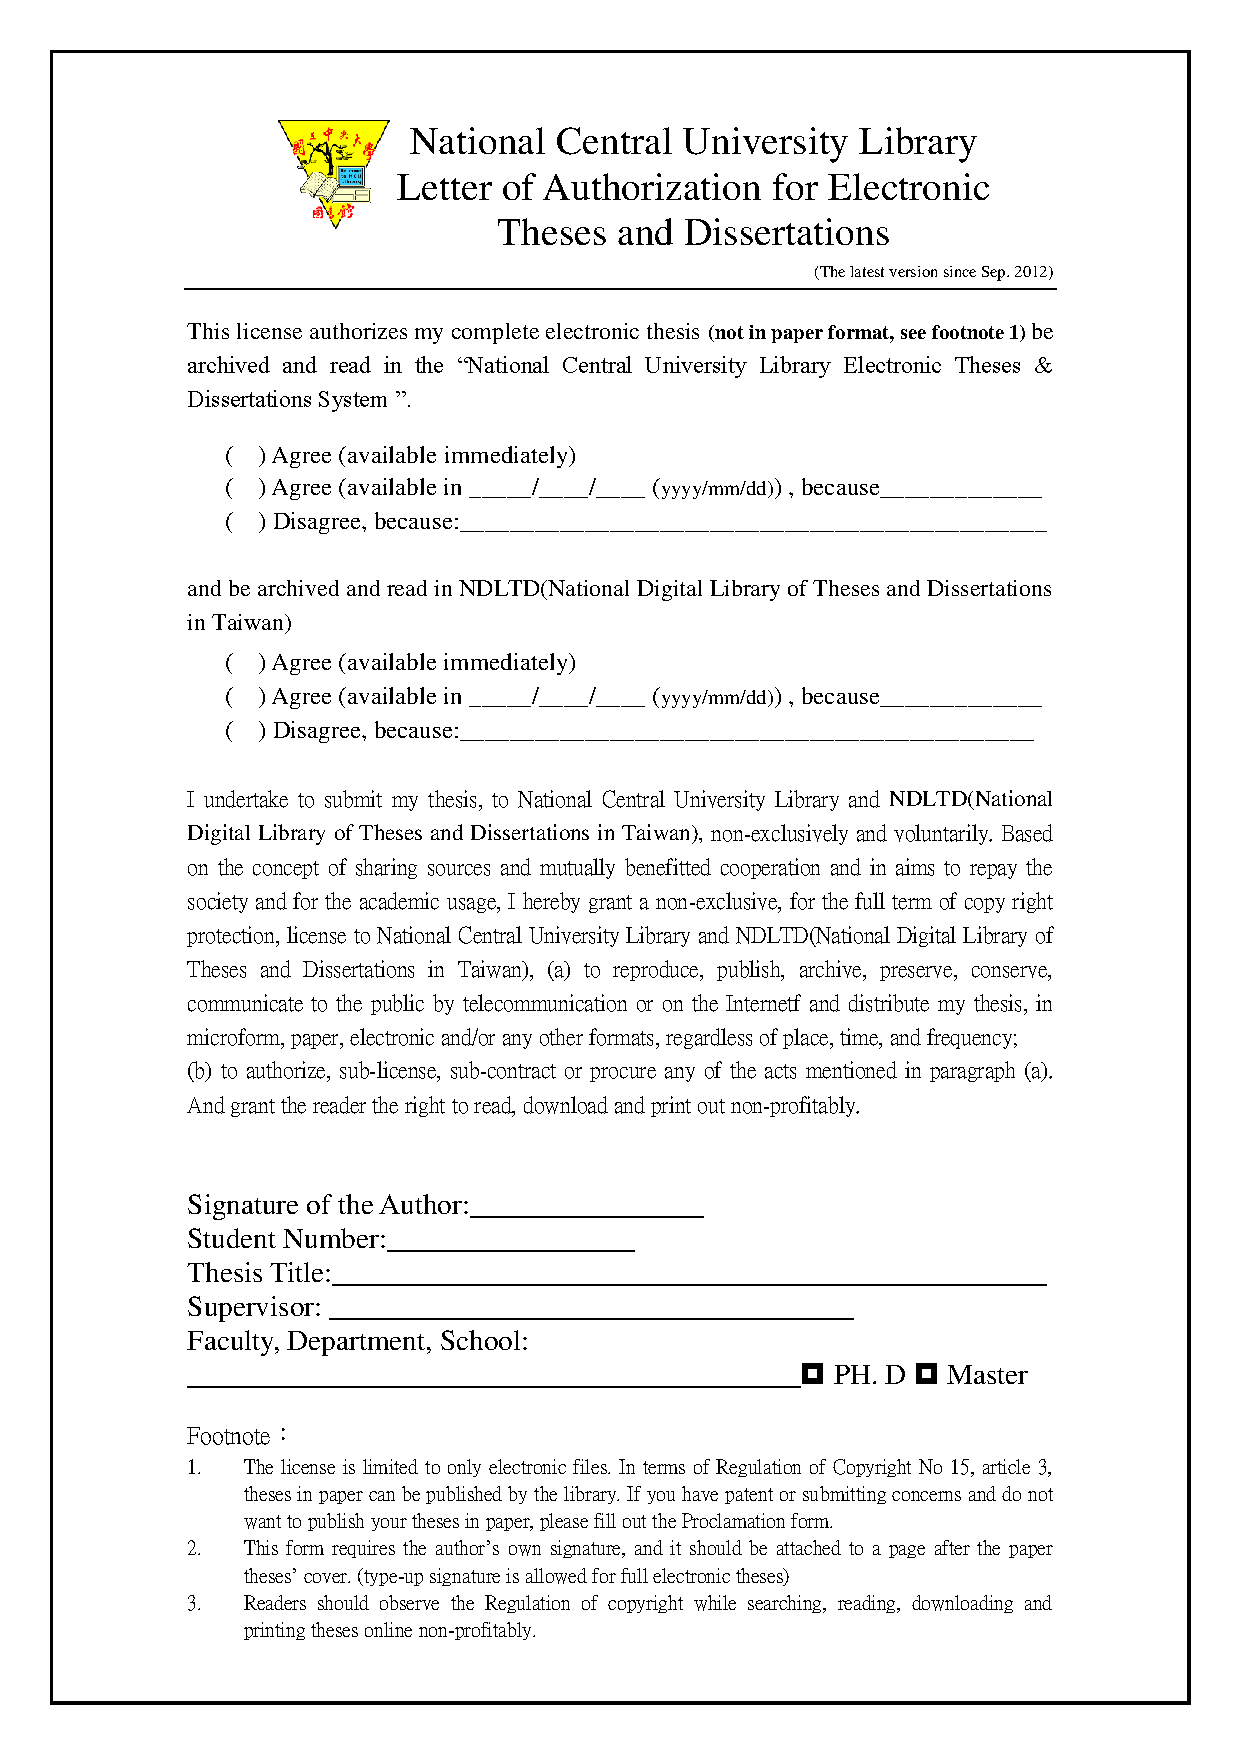
\includepdf{letter_authorization.pdf}}{}
        % 碩博士紙本論文延後公開/下架申請書(可略)。 Publication request (option)
        \IfFileExists{letter_publication_request.pdf}{
            \cleardoublepage
            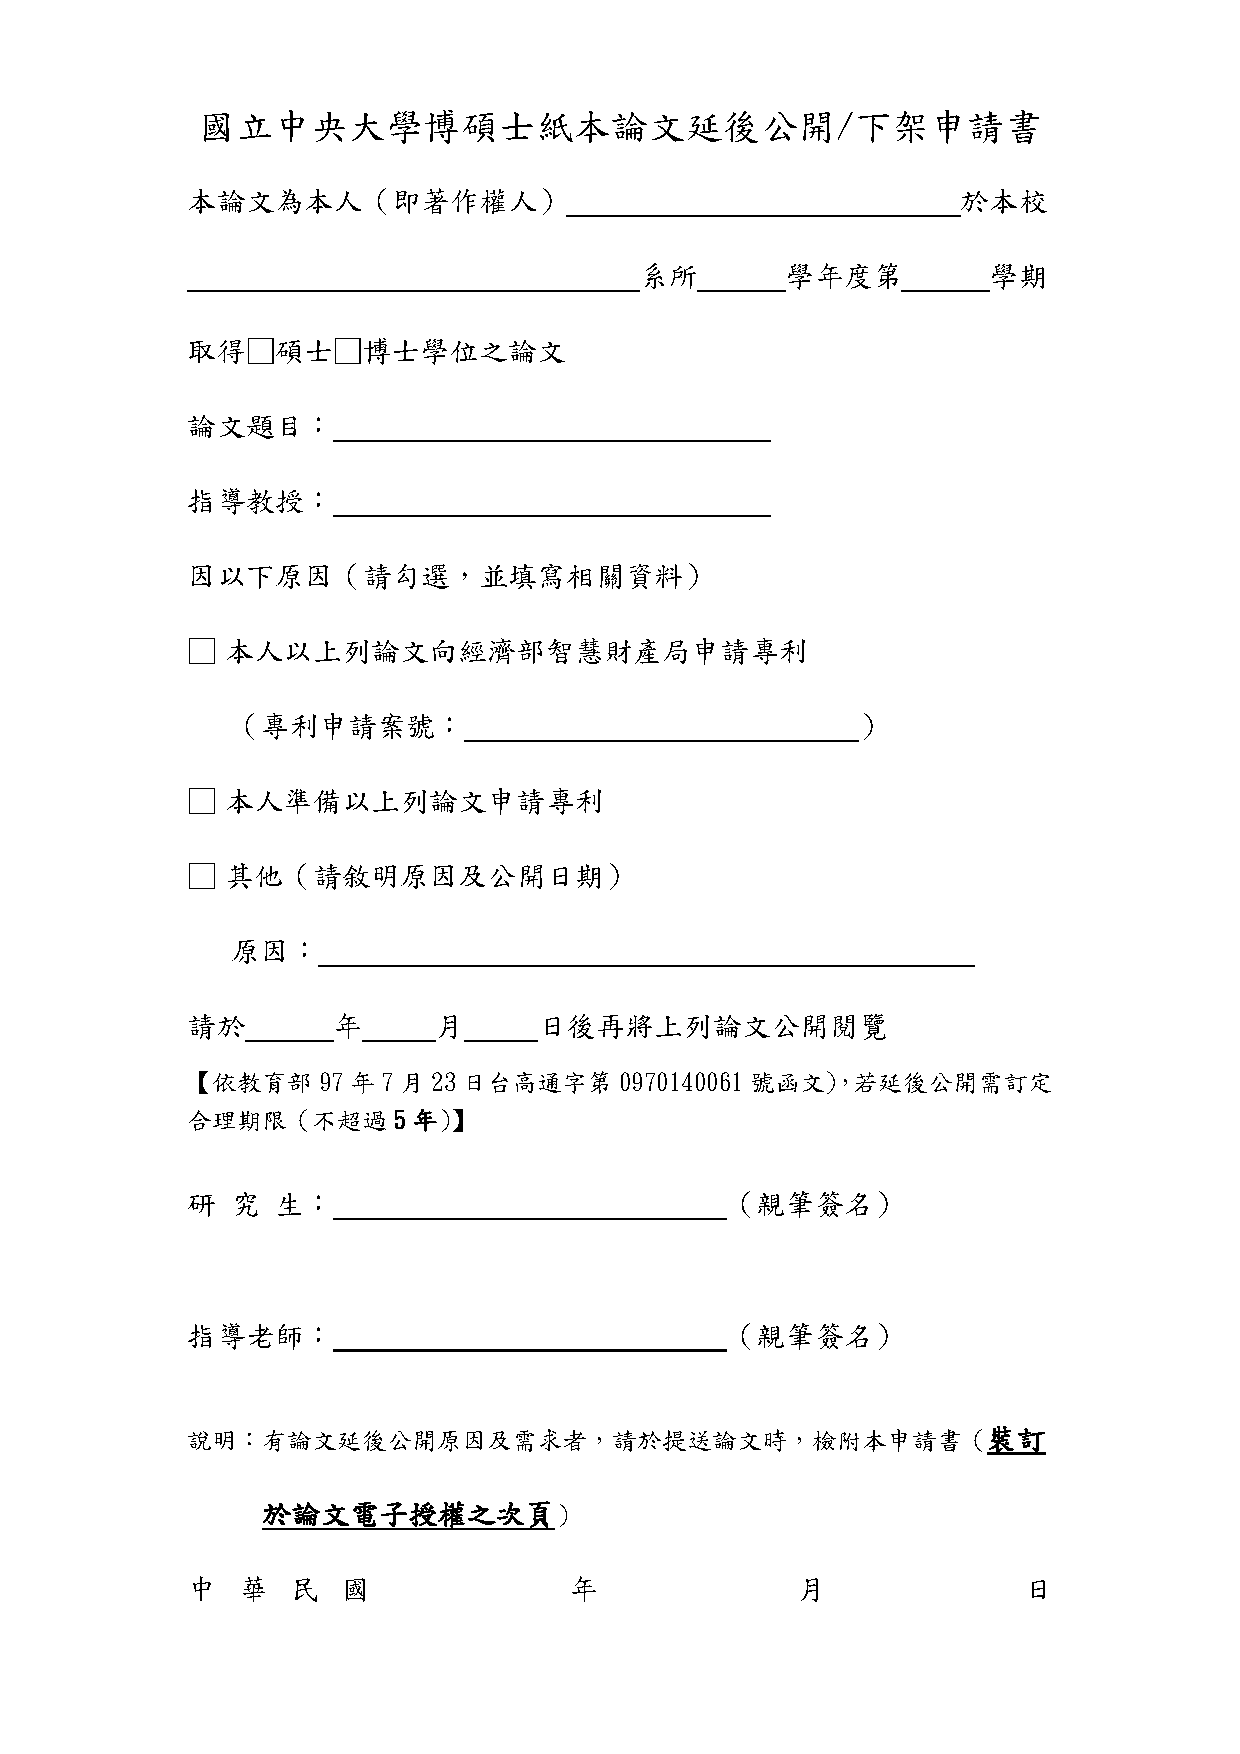
\includepdf{letter_publication_request.pdf}}{}
        % 指導教授推薦書
        \IfFileExists{letter_recommendation.pdf}{
            \cleardoublepage
            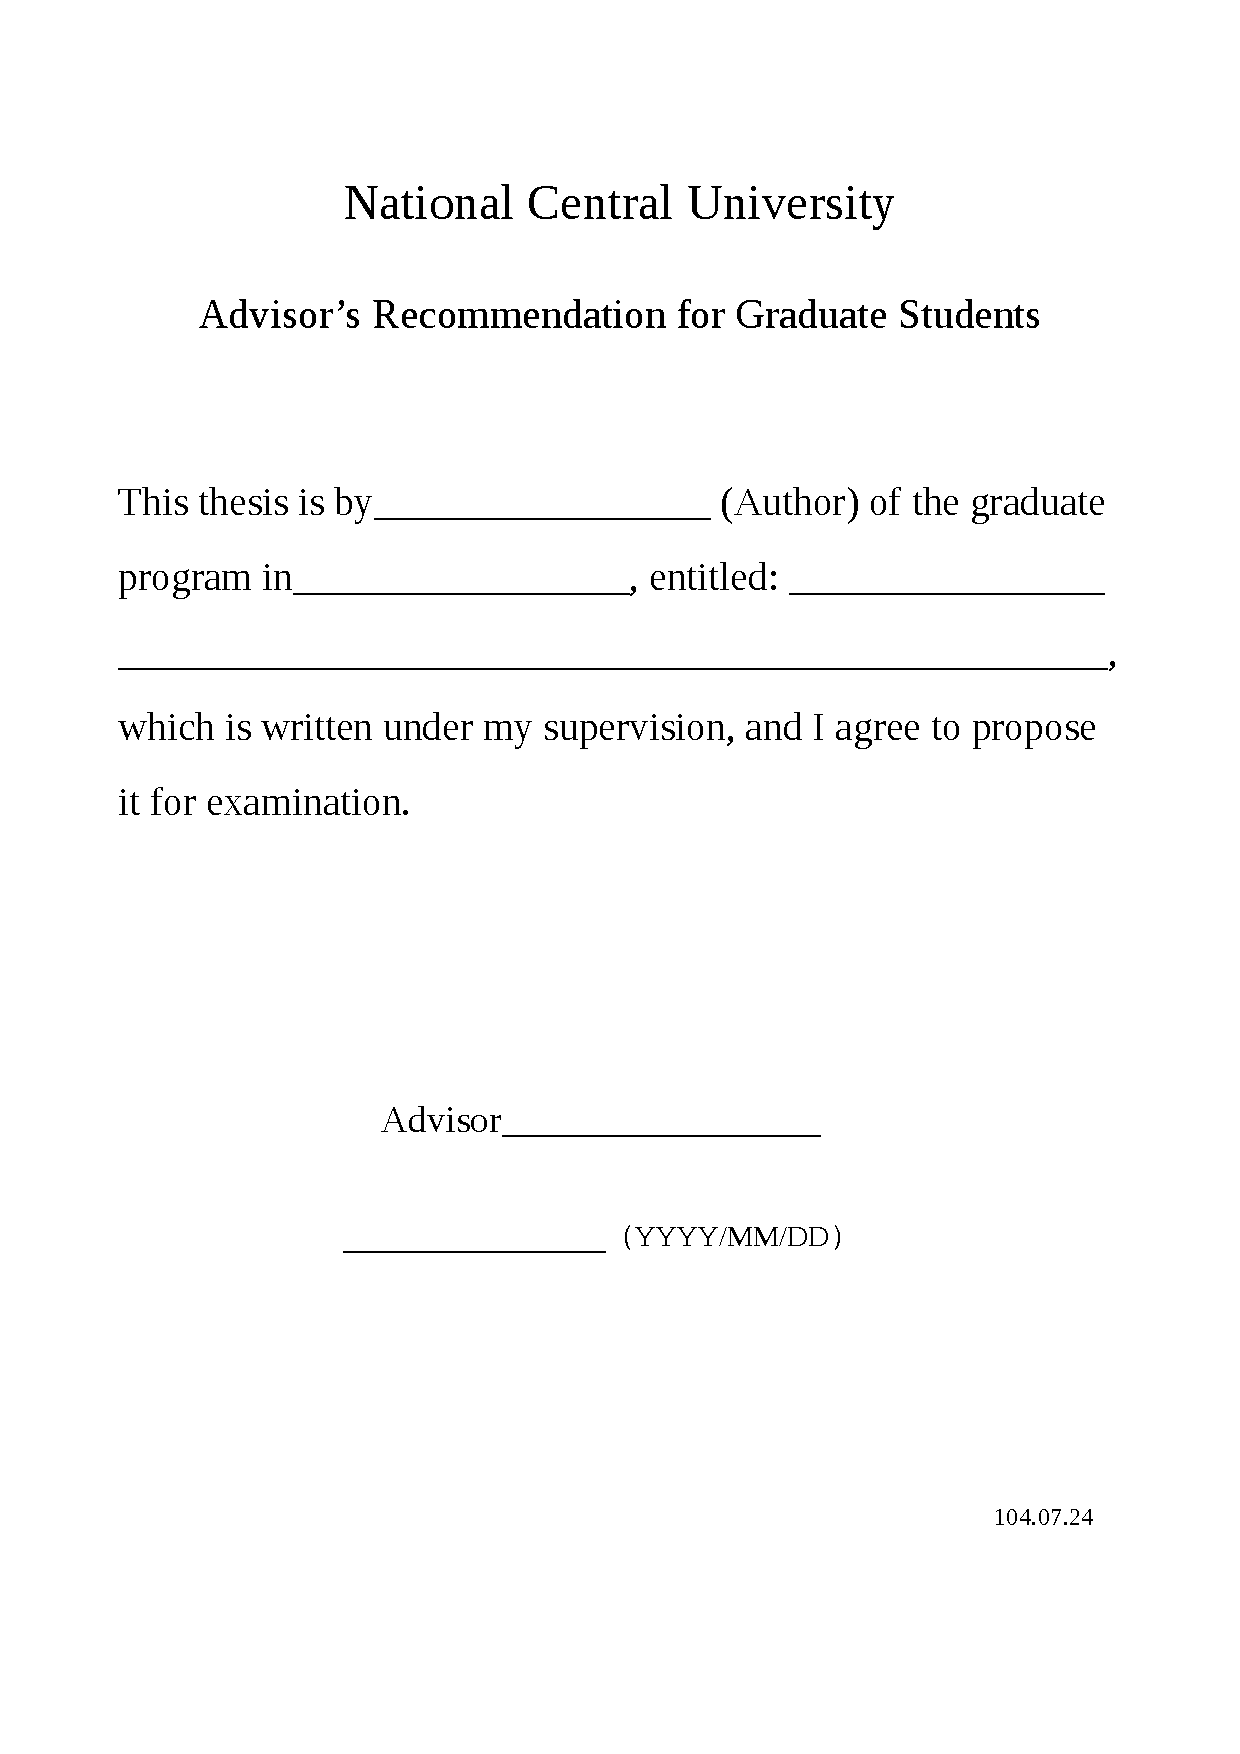
\includepdf{letter_recommendation.pdf}}{}
        % 口試委員審定書
        \IfFileExists{letter_verification.pdf}{
            \cleardoublepage
            
\includepdf{letter_verification.pdf}}{}
        \cleardoublepage
        % 中英文論文摘要:內容應說明研究目的,資料來源,研究方法及研究結果等
        \ifthenelse{\boolean{disableChinese} \OR \NOT \equal{\titlepageLang}{zh} \AND \NOT \equal{\titlepageLang}{en}}{
            \renewcommand\thispage{Chinese abstract}
            \documentclass[class=NCU_thesis_en, crop=false]{standalone}
\begin{document}

\fontsize{16}{25}\selectfont
% --------define title page layout for thesis
\sffamily % use sans font
\newgeometry{top=2.5cm, bottom=2.5cm, inner=2cm, outer=2cm} % only for titlepage
\begin{titlepage}
    \vspace*{30mm}
    \begin{center}
        {\Huge\textbf{\thispage\ hidden now !!}\par}
    \end{center}
    \vspace*{30mm}
    {\Huge 
    It avoid you get error because your computer no Chinese font, 
    Please set ``titlepageLang'' value (to zh or en) in the ``config.tex'' to display this page.
    if you don't have Chinese font, you can try ``cwTeX'' font. 
    (\url{https://github.com/l10n-tw/cwtex-q-fonts})\par}
    \null\vfill
\end{titlepage}
\restoregeometry
\rmfamily % use main font
%--------end of title page for thesis
\cleardoublepage
\end{document}

        }{
            \documentclass[class=NCU_thesis, crop=false]{standalone}
\begin{document}

\chapter{摘要}
在此寫上你的中文摘要。

\vspace{2em}
\noindent \textbf{關鍵字:} \keywordsZh{} % Set keywords in config.tex
\end{document}
        }
        \documentclass[class=NCU_thesis, crop=false, float=true]{standalone}
\begin{document}
% This file is common document region, 
% it will loading when LaTeX see ``\begin{document}'' 
% It's for some command which need use in document region.
% DON'T put preamble only command in here, eg. \usepackage
% --------------------------------------------------

% standalone setting for sub-tex. (not every class option can use \standaloneconfig)
\IfStandalone{\standaloneconfig{float=true}}{} 
% ``float=false'' disable floating environment when build sub-tex.

% Old method for change font size, but no limit for size so keep here.
% \fontsize{size}{baselineskip} 無級調大小、行高, 行高倍數 = baselineskip/size/1.2 ,詳見教學。
% \fontsize{14}{25}\selectfont  

\ifzh{
    \setlength{\parindent}{2em} % 中文段首縮排2中文字寬
}{}                             % 英文照 LaTeX 預設


\chapter{Abstract}
Write your English abstract here.



\vspace{2em}
\noindent \textbf{Keywords:} \keywordsEn{} % Set keywords in config.tex
\end{document} % English abstract
        \documentclass[class=NCU_thesis, crop=false]{standalone}
\begin{document}

\chapter{誌謝}

感謝中央大學、中央研究院提供的資源。Donald Ervin Knuth 的 \TeX\ ,Linus與眾多自由軟體好手提供的GNU/Linux。
另外特別感謝sppmg提供的論文樣板與教學\cite{_sppmg/tw_thesis_template_????},
讓我將學習\LaTeX\ 的時間拿來充實論文內容。(以上為sppmg自肥 XD)

\begin{figure}[!hbt]
    \captionsetup[subfigure]{labelformat=empty}
    \centering
    \subcaptionbox
        {}
        {
\includegraphics[width=0.2\linewidth]{logo-NCU.jpg}}
    ~
    \subcaptionbox
        {}
        {
\includegraphics[width=0.2\linewidth]{logo-sinica.png}}
    ~
    \subcaptionbox
        {}
        {
\includegraphics[width=0.2\linewidth]{logo-GNU.png}}
    ~
    \subcaptionbox
        {}
        {
\includegraphics[width=0.2\linewidth]{logo-Linux.png}}
    % \vspace{\baselineskip} % 分隔上下列	
\end{figure}


\end{document}


 % acknowledgements(option) 誌謝(可略)
            \cleardoublepage
            \phantomsection
            \addcontentsline{toc}{chapter}{Contents}    % Add ``Contents'' to TOC
        \tableofcontents        % Table Of Contents
        \listoffigures          % List Of Figures   圖目錄
        \listoftables           % List Of Tables    表目錄
        \documentclass[class=NCU_thesis, crop=false]{standalone}
\begin{document}

\chapter{Symbol}
Use table for symbol list

\begin{table}[h]
	\fontsize{14}{25}\selectfont  % 使用與內文一樣大的字體,請自調
	\centering
	\begin{tabular}{c@{\quad}@{:}l}
% 		符號		& \ 說明 \\ 
		VIM     & The best guy's editor \\ 
		Emacs   & The God's editor \\ 
		CTAN    & Comprehensive TeX Archive Network, ctan.org \\
		
	\end{tabular} 
	\caption{Symbols} % Hide caption by comment/remove it, label will inactive also. 不想顯示請註解/刪除\caption行(\label自動失效)
	\label{table:symbol_def}
\end{table}

\end{document}
    % Symbols           符號及術語
    \mainmatter
        \documentclass[class=NCU_thesis, crop=false]{standalone}
\begin{document}


\chapter{Introduction}
(You can copy ``chapter\_template.tex'' or ``chapter\_template\_demo.tex'' to create new sub-file(chapter). )

Write your Introduction here.
eg, \\
I don't want my chaste thesis impinge by M\${}. But \LaTeX\ is little hard.

\end{document}    % introduction  緒論
        \documentclass[class=NCU_thesis, crop=false, float=true]{standalone}
\begin{document}
% This file is common document region, 
% it will loading when LaTeX see ``\begin{document}'' 
% It's for some command which need use in document region.
% DON'T put preamble only command in here, eg. \usepackage
% --------------------------------------------------

% standalone setting for sub-tex. (not every class option can use \standaloneconfig)
\IfStandalone{\standaloneconfig{float=true}}{} 
% ``float=false'' disable floating environment when build sub-tex.

% Old method for change font size, but no limit for size so keep here.
% \fontsize{size}{baselineskip} 無級調大小、行高, 行高倍數 = baselineskip/size/1.2 ,詳見教學。
% \fontsize{14}{25}\selectfont  

\ifzh{
    \setlength{\parindent}{2em} % 中文段首縮排2中文字寬
}{}                             % 英文照 LaTeX 預設


\chapter{實驗方法及裝置}
為了防止世界被破壞$\sim$ \\
為了守護世界的和平$\sim$

\end{document}          % method        分析方法
        \documentclass[class=NCU_thesis, crop=false, float=true]{standalone}
\begin{document}
% This file is common document region, 
% it will loading when LaTeX see ``\begin{document}'' 
% It's for some command which need use in document region.
% DON'T put preamble only command in here, eg. \usepackage
% --------------------------------------------------

% standalone setting for sub-tex. (not every class option can use \standaloneconfig)
\IfStandalone{\standaloneconfig{float=true}}{} 
% ``float=false'' disable floating environment when build sub-tex.

% Old method for change font size, but no limit for size so keep here.
% \fontsize{size}{baselineskip} 無級調大小、行高, 行高倍數 = baselineskip/size/1.2 ,詳見教學。
% \fontsize{14}{25}\selectfont  

\ifzh{
    \setlength{\parindent}{2em} % 中文段首縮排2中文字寬
}{}                             % 英文照 LaTeX 預設


\chapter{實驗結果}

\centering 

可愛又迷人的反派角色  \\
武藏! \\
小次郎! \\
我們是穿梭在銀河中的火箭隊 \\
白洞、白色的明天正等著我們 \\

\end{document}          % result        實驗結果
        \documentclass[class=NCU_thesis, crop=false, float=true]{standalone}
\begin{document}
% This file is common document region, 
% it will loading when LaTeX see ``\begin{document}'' 
% It's for some command which need use in document region.
% DON'T put preamble only command in here, eg. \usepackage
% --------------------------------------------------

% standalone setting for sub-tex. (not every class option can use \standaloneconfig)
\IfStandalone{\standaloneconfig{float=true}}{} 
% ``float=false'' disable floating environment when build sub-tex.

% Old method for change font size, but no limit for size so keep here.
% \fontsize{size}{baselineskip} 無級調大小、行高, 行高倍數 = baselineskip/size/1.2 ,詳見教學。
% \fontsize{14}{25}\selectfont  

\ifzh{
    \setlength{\parindent}{2em} % 中文段首縮排2中文字寬
}{}                             % 英文照 LaTeX 預設


\chapter{總結}
就是這樣,喵!

\end{document}      % conclusion    結論
        \documentclass[class=NCU_thesis, crop=false, float=true]{standalone}

\begin{document}
% This file is common document region, 
% it will loading when LaTeX see ``\begin{document}'' 
% It's for some command which need use in document region.
% DON'T put preamble only command in here, eg. \usepackage
% --------------------------------------------------

% standalone setting for sub-tex. (not every class option can use \standaloneconfig)
\IfStandalone{\standaloneconfig{float=true}}{} 
% ``float=false'' disable floating environment when build sub-tex.

% Old method for change font size, but no limit for size so keep here.
% \fontsize{size}{baselineskip} 無級調大小、行高, 行高倍數 = baselineskip/size/1.2 ,詳見教學。
% \fontsize{14}{25}\selectfont  

\ifzh{
    \setlength{\parindent}{2em} % 中文段首縮排2中文字寬
}{}                             % 英文照 LaTeX 預設


\chapter{章名(章節示例)}
章內容
\section{節名}
節內容
\subsection{小節名}
 \subsubsection{小小節}
 \paragraph{段}


\chapter{文字}
第一行。
仍是第一行。 \\
第二行。


\chapter{圖片}
\subsection{插入單一圖片}
\insfig[0.15][fig:labal_test][!hbt]{logo-Linux.png}[caption][short caption]

\subsection{插入多張圖片}
\begin{figure}[!hbt]
    %\captionsetup[subfigure]{labelformat=empty} % 完全隱藏圖號
    \centering
    \subcaptionbox
        {Linux (A kernel of OS)
        \label{fig:subfig_linux}}
        {
\includegraphics[width=0.3\linewidth]{logo-Linux.png}}
    ~
    \subcaptionbox
        {Debain (A popular distribution). Demo long caption,  bla bla bla bla bla.
        \label{fig:subfig_debian}}
        {
\includegraphics[width=0.3\linewidth]{logo-Debian.png}}
    \vspace{\baselineskip} % 分隔上下列
    \subcaptionbox
        {GNU (A project of OS)
        \label{fig:subfig_gnu}}
        {
\includegraphics[width=0.6\linewidth]{logo-GNU.png}}
     % use ``\subref{fig:subfig_debian}'' get ID of subfigure(this ID is Debian)
    \caption{caption, 使用 \subref{fig:subfig_debian}取得子圖(Debian)編號 }
    \label{fig:labal}
\end{figure}


\chapter{表格}
\subsection{一般表格}
\begin{table}[h]
    \centering
    \caption{Solution}
    \begin{tabular}{| l | l |}
        \hline
        Component & Concentration(mM) \\ \hline
        \ce{NaCl} & 118.0 \\ \hline
    \end{tabular}
\end{table}

\subsection{自動折行表格}
\begin{table}[h]
    \centering
    \begin{tabularx}{\textwidth}{| l | X |}
        \hline
        short & short short \\ \hline
        long & long long long long long long long long long long \\ \hline
    \end{tabularx}
\end{table}

\end{document}   % some demo
    \backmatter          % book class 預設\backmatter 在\appendix 後面。因此.cls修改過\appendix 定義
        \printbibliography[heading = bibnumbered]
    \appendix
        % device list
\documentclass[class=NCU_thesis, crop=false, float=true]{standalone}
\begin{document}
% This file is common document region, 
% it will loading when LaTeX see ``\begin{document}'' 
% It's for some command which need use in document region.
% DON'T put preamble only command in here, eg. \usepackage
% --------------------------------------------------

% standalone setting for sub-tex. (not every class option can use \standaloneconfig)
\IfStandalone{\standaloneconfig{float=true}}{} 
% ``float=false'' disable floating environment when build sub-tex.

% Old method for change font size, but no limit for size so keep here.
% \fontsize{size}{baselineskip} 無級調大小、行高, 行高倍數 = baselineskip/size/1.2 ,詳見教學。
% \fontsize{14}{25}\selectfont  

\ifzh{
    \setlength{\parindent}{2em} % 中文段首縮排2中文字寬
}{}                             % 英文照 LaTeX 預設


\chapter{裝置列表}

\begin{table}[!h]
    \centering
    \begin{tabularx}{\textwidth}{|l|l|X|}
        \hline
        裝置	     & 型號      & 說明 \\ \hline
        Linux    & Debian 9 & 世界好用的作業系統 \\ \hline
        Windows  & 10       & 防止人腦老化的工具 \\ \hline
    \end{tabularx}
    \caption{裝置列表}
    \label{table:list_device}
\end{table}

\end{document}
        \documentclass[class=NCU_thesis_en, crop=false]{standalone}
\begin{document}

\definecolor{Gray3}{gray}{0.8}

\chapter{Solutions}

\section{The solution}
\begin{table}[!h]
    \centering
    \begin{tabular}{| l | l |}
        \hline
        Component & Concentration(mM) \\ \hline
        \rowcolor{Gray3}
        \ce{NaCl} & 1.0 \\ \hline
        \ce{CaCl_2} & 2.0 \\ \hline
        \rowcolor{Gray3}
        \ce{NaCl} & 1.0 \\ \hline
        \ce{CaCl_2} & 2.0 \\ \hline
    \end{tabular}
    \caption{The solution}
\end{table}
\end{document}
        \documentclass[class=NCU_thesis, crop=false]{standalone}
\begin{document}
% Here demo instert whole code file. You can only insert code directly, 
% please read my tutorial or document of listings package.
% code style set in macros_preamble already.
% Supported language please read document of listings package.

\chapter{程式碼}
\section{C}
\lstinputlisting[language=C]{hello_world_c.c}

\section{Matlab}
\lstinputlisting[language=matlab]{hello_world_matlab.m}

\section{IDL}
\lstinputlisting[language=IDL]{hello_world_idl.pro}
\end{document}

        
        \ifthenelse{\boolean{disableChinese} \OR \NOT \equal{\titlepageLang}{zh} \AND \NOT \equal{\titlepageLang}{en}}{
            \renewcommand\thispage{Automatical write letters}
            \documentclass[class=NCU_thesis_en, crop=false]{standalone}
\begin{document}

\fontsize{16}{25}\selectfont
% --------define title page layout for thesis
\sffamily % use sans font
\newgeometry{top=2.5cm, bottom=2.5cm, inner=2cm, outer=2cm} % only for titlepage
\begin{titlepage}
    \vspace*{30mm}
    \begin{center}
        {\Huge\textbf{\thispage\ hidden now !!}\par}
    \end{center}
    \vspace*{30mm}
    {\Huge 
    It avoid you get error because your computer no Chinese font, 
    Please set ``titlepageLang'' value (to zh or en) in the ``config.tex'' to display this page.
    if you don't have Chinese font, you can try ``cwTeX'' font. 
    (\url{https://github.com/l10n-tw/cwtex-q-fonts})\par}
    \null\vfill
\end{titlepage}
\restoregeometry
\rmfamily % use main font
%--------end of title page for thesis
\cleardoublepage
\end{document}

        }{
            \documentclass[class=NCU_thesis, crop=false]{standalone}

\NewDocumentCommand{\ffs}{m}{\fontsize{#1}{#1}\selectfont}

\begin{document}
\chapter{自動填單}
這裡試著幫各位自動填入部份資訊,其餘打勾、日期請手寫。有字體大小不符、位置歪掉等問題的話,請修改 appendix\_letter\_NCU.tex後直接編譯生成文件。

appendix\_letter\_NCU.tex中,每個句子(文字項目)都是獨立的大小與位置。 大小可由\textbackslash{}ffs,調整。
\footnote{\textbackslash{}ffs 使用 \textbackslash{}fontsize 做無級調整,並固定單行高度。 }
位置可由\textbackslash{}placetextbox 調整。語法如下:
\begin{lstlisting}[style=LatexStyle,caption={}]
\placetextbox{x(mm)}{y(mm)}
\end{lstlisting}
單位使用mm ,(0,0)位於左下角。建議調整時將``grid''加入documentclass選項。(加入子檔的即可)
\begin{lstlisting}[style=LatexStyle,caption={}]
\documentclass[class=NCU_thesis, crop=false, grid]{standalone}
\end{lstlisting}
grid 將顯示格線(一小格是\SI{5}{\milli\metre})。

\begin{center}
{ \noindent\color{red}\bfseries\Large 目前僅提供碩士論文所需的中文文件}
\end{center}

%%%%%%%%%%%%%%%%%%%%%%%%%%%%%%%%
\cleardoublepage
\pagestyle{empty}
\sffamily
% ------------------------------

% % 碩博士論文電子檔授權書
\IfFileExists{letter_authorization.pdf}{
\cleardoublepage\thispagestyle{empty}
\includepdf[pagecommand={   \placetextbox{100}{120}{\ffs{17}\title}%
                            \placetextbox{95}{109}{\ffs{17}\mprof}%
                            \placetextbox{69}{98}{\ffs{17}\deptshort} }]%
{letter_authorization.pdf}}{}

% 碩博士紙本論文延後公開/下架申請書。(如需延後公開者,才需要裝訂於論文內頁)
\IfFileExists{letter_publication_request.pdf}{
\cleardoublepage\thispagestyle{empty}
\includepdf[pagecommand={   \placetextbox{128}{270}{\ffs{17}\author}%
                            \placetextbox{70}{258}{\ffs{17}\deptshort}%
                            \placetextbox{100}{233}{\ffs{17}\title}%
                            \placetextbox{90}{219.3}{\ffs{17}\mprof} }]%
{letter_publication_request.pdf}}{}

% 指導教授推薦書
\IfFileExists{letter_recommendation.pdf}{
\cleardoublepage\thispagestyle{empty}
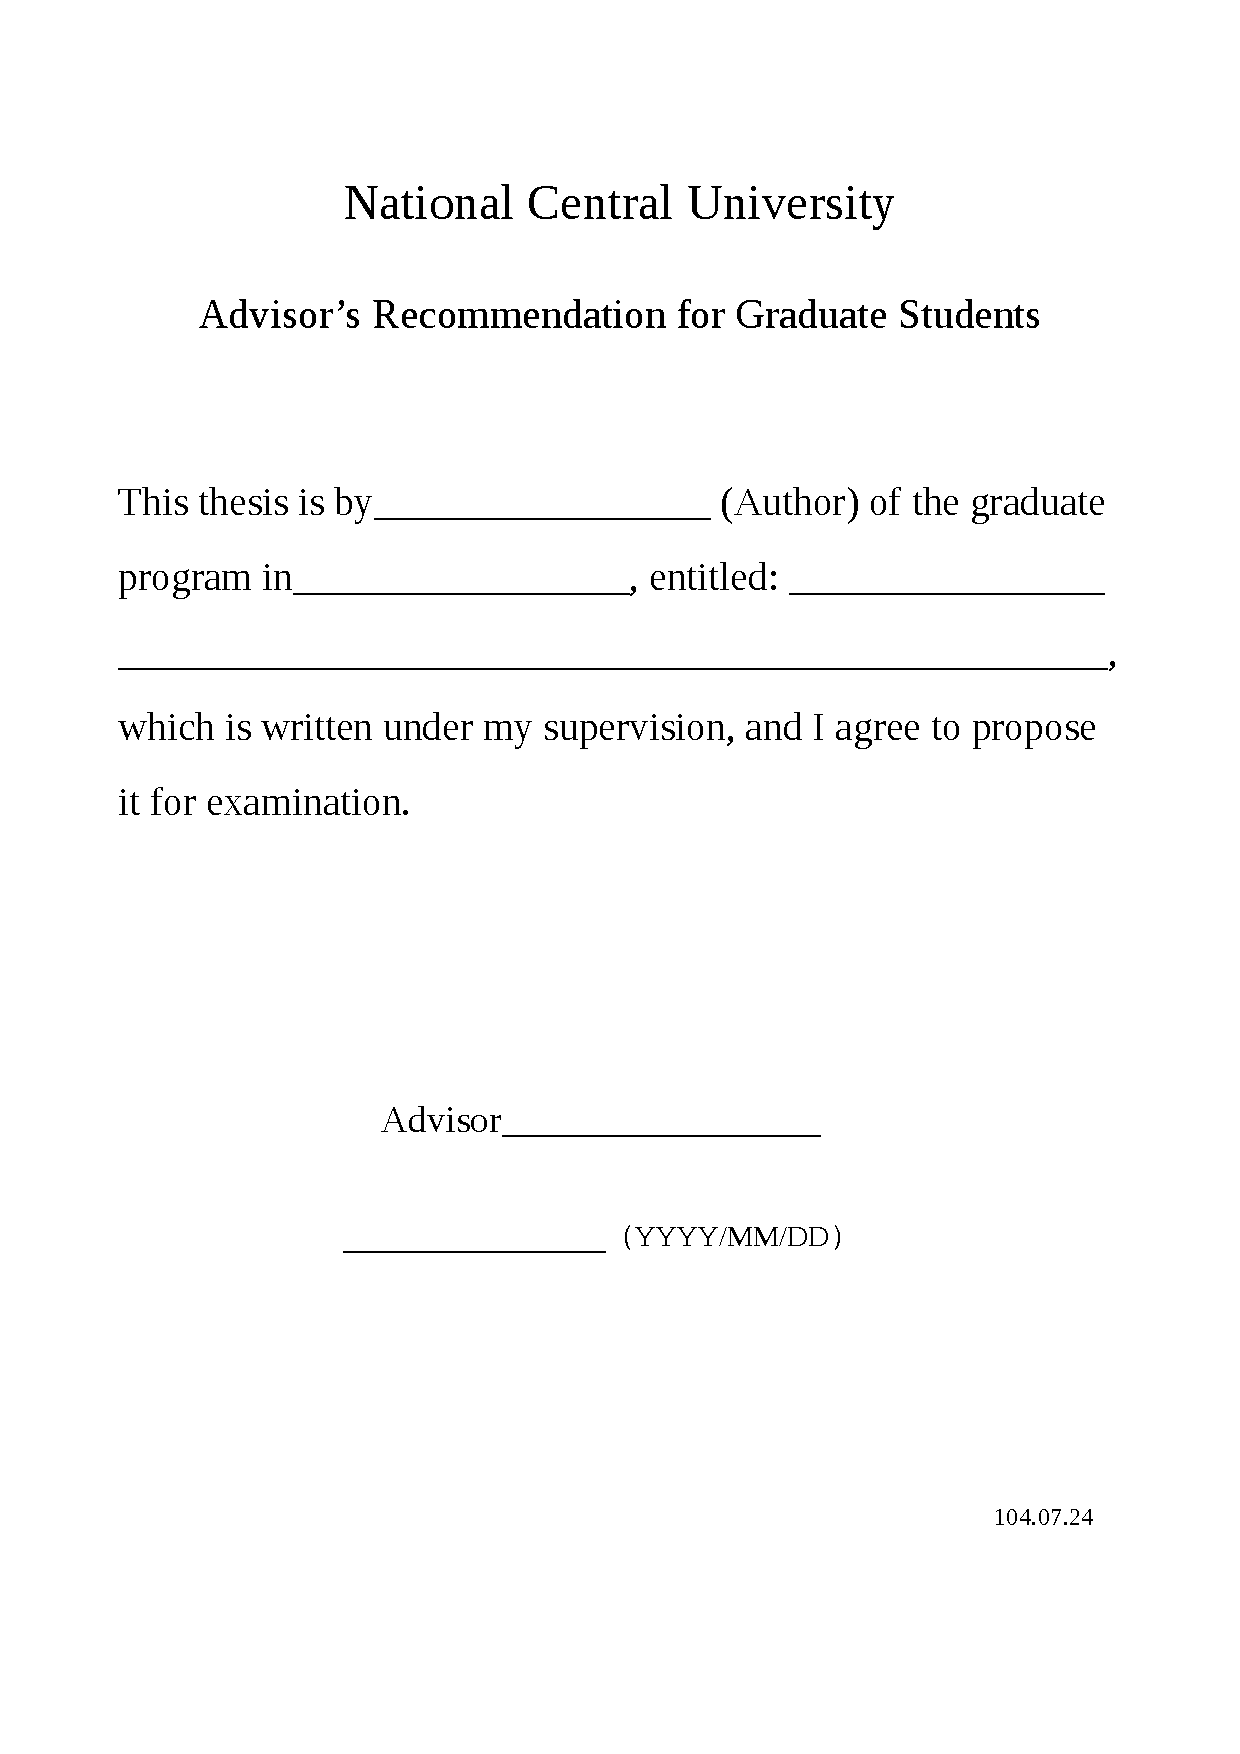
\includepdf[pagecommand={   \placetextbox{50}{159}{\ffs{22}\deptshort}%
                            \placetextbox{118}{159}{\ffs{22}\author}%
                            \placetextbox{105}{144}{\ffs{22}\title}}%
]{letter_recommendation.pdf}}{}

% 口試委員審定書
\IfFileExists{letter_verification.pdf}{
\cleardoublepage\thispagestyle{empty}

\includepdf[pagecommand={   \placetextbox{63}{200.5}{\ffs{22}\deptshort}%
                            \placetextbox{145}{200.5}{\ffs{22}\author}%
                            \placetextbox{100}{170}{\ffs{22}\title}}%
]{letter_verification.pdf}}{}

% ------------------------------
\pagestyle{fancy}
\end{document}
        }
\end{document}